\documentclass[border=3pt]{standalone}
\usepackage{tikz}

\begin{document}
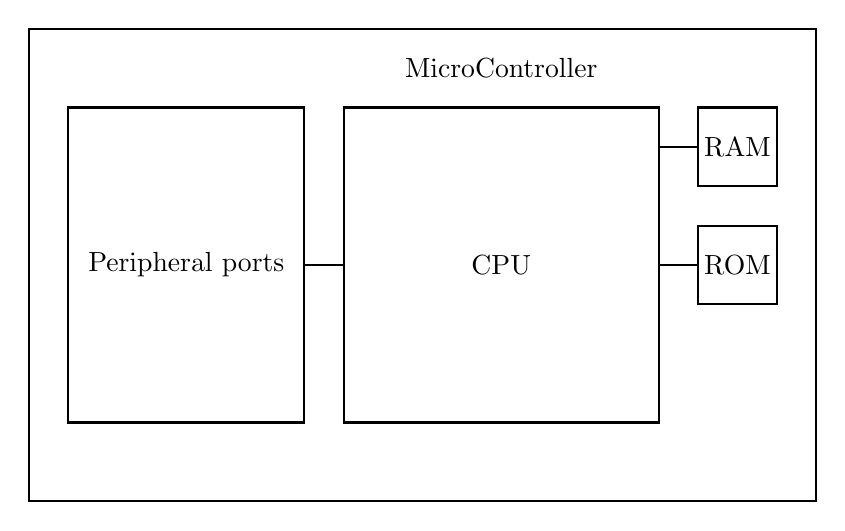
\begin{tikzpicture}

    \draw[thick] (0, 0) rectangle (10, 6);

    \draw[thick] (0.5, 1) rectangle (3.5, 5);
    \node at (2, 3) {Peripheral ports};

    \draw[thick] (4, 1) rectangle (8, 5);
    \node at (6, 3) {CPU};

    \draw[thick] (8.5, 4) rectangle (9.5, 5);
    \node at (9, 4.5) {RAM};

    \draw[thick] (8.5, 2.5) rectangle (9.5, 3.5);
    \node at (9, 3) {ROM};

    \draw[thick] (3.5, 3) -- (4, 3);
    \draw[thick] (8, 4.5) -- (8.5, 4.5);
    \draw[thick] (8, 3) -- (8.5, 3);

    \node at (6, 5.5) {MicroController};

\end{tikzpicture}
\end{document}
